\section{CMOS}
Most recent update: 2016-12-02 \\
Contact person: Marc Winter (email: marc.winter@iphc.cnrs.fr)

\subsection{Introduction}
CMOS Pixel Sensors (CPS) combine high granularity with low material
budget and allow integrating the full signal processing circuitry on
the sensor substrate. Being moreover cost effective because of the
underlying industrial market, CPS are attractive for a wide range of
applications. They are developed for the ILC since more than fifteen
years and were shown to rather easily comply with the required spatial
resolution and material budget of an ILC vertex detector and their
radiation tolerance was observed to go well beyond the ILC requirements~\cite{Behnke:2013lya}. The state of the art of the technology is illustrated
by the 400 ULTIMATE sensors operated in the STAR-PXL detector~\cite{Greiner201168}
at RHIC/BNL since 2014 and by the 10 -- 100 times faster
sensors developed for the upgrade of the ALICE Inner Tracker System
(ITS)~\cite{0954-3899-41-8-087002}.

\begin{figure}
	\centering
	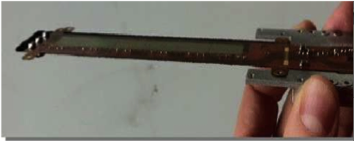
\includegraphics[width=.5\linewidth]{VertexDetector/CMOS/Ladder}
	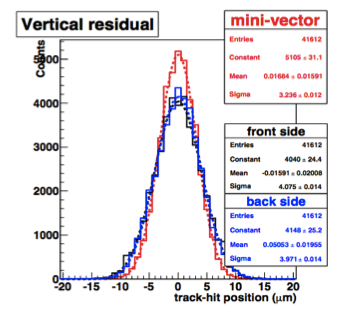
\includegraphics[width=.34\linewidth]{VertexDetector/CMOS/trackResolution.png}
	\caption{left: Photograph of a MIMOSA ladder for EUDET. right: A track resolution of \SI{3}{\micro\meter} has been achieved.}
	\label{fig:VertexDetector:CMOS}
\end{figure}

\begin{figure}
	\centering
	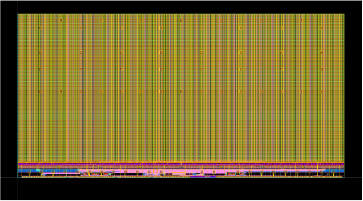
\includegraphics[width=.45\linewidth]{VertexDetector/CMOS/Mistral}
	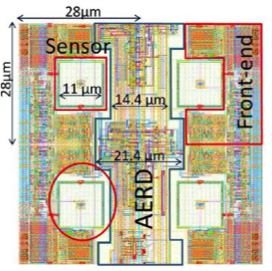
\includegraphics[width=.35\linewidth]{VertexDetector/CMOS/ALPIDE}
	\caption{Two architectures are being developed: Left: synchronous readout in the MISTRAL chip. Right: asynchronous readout in the ALPIDE chip}
	\label{fig:VertexDetector:CMOS:architectures}
\end{figure}

\begin{figure}
	\centering
	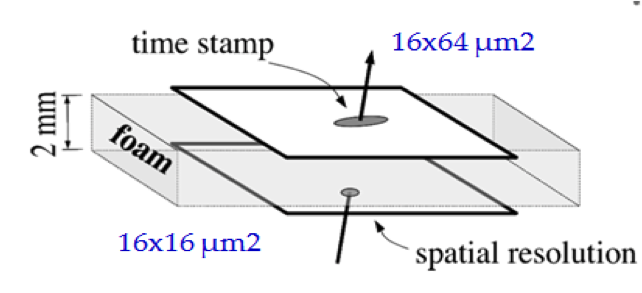
\includegraphics[width=.5\linewidth]{VertexDetector/CMOS/doubleSided}
	\caption{Double-sided ladders: mini-vectors providing
      high spatial resolution and time stamping}
	\label{fig:VertexDetector:CMOS:doubleSided}
\end{figure}

The achieved read-out speed of the CPS developed for an ILC
vertex detector is already quite satisfactory~\cite{Behnke:2013lya},
but is worth
improving in order to facilitate track seeding at nominal ILC
running conditions and to introduce a safety margin reflecting the
uncertainties affecting the predicted beam related background rate.

The technology should in fact allow single bunch tagging, provided power
consumption and, in turn, power cycling remain under control. The flexibility and detection performances of CPS are also indicating attractive perspectives for trackers, where relaxed constraints on the granularity may be exploited
to find a well suited balance between speed, power saving and material budget. Ambitious goals for an ILC experiment may therefore be considered
since their development may be carried out for numerous years until the design
inputs of a vertex detector ought to be fixed.

The charged particle detection performances of CPS are
currently essentially limited by manufacturing parametres.
The latter evolve steadily since several years in a direction which makes
them increasingly suited to the ILC vertexing and tracking. Besides
achievements targetted with existing processes, the present R\&D
addresses also improvements expected from the evolution of the CMOS
industry, mainly driven by the trend towards smaller feature sizes which
would allow overcoming the conflict between the spatial resolution and the
bunch tagging capability of CPS. This evolution is already well visible
when comparing the performances achieved with the $\SI{0.35}{\mu m}$ process
used for the STAR-PXL and the more recently addressed $\SI{0.18}{\mu m}$ process
used for the ALICE experiment.


The R\&D adresses presently four objectives :
\begin{itemize}
\item 2 or 3 CPS variants optimised for the different vertex detector layers :
\begin{itemize}
\item inner layer : design privileging spatial resolution and read-out speed
\item outer layers : design privileging power saving, exploiting the
				less demanding spatial and time resolutions
\end{itemize}
\item CPS adapted to tracking sub-systems, based on large pixels and privileging
power saving
\item ultra-light double sided ladders (called PLUME~\cite{Nomerotski2011208})
equipped with (identical or complementary) CPS on its two faces
\end{itemize}


\subsection{Recent Milestones}
Specific CPS are being developed since 2011 to equip the Inner Tracking
System (ITS) of the ALICE experiment in the framework of its upcoming
upgrade. The surface to cover exceeds 10 square meters, i.e. nearly two
ordres of magnitude more than the STAR-PXL or an ILC vertex detector.

Two CPS are being developed, differing by their read-out architectures.
The most conservative of them, called MISTRAL-0, reproduces the ULTIMATE
sensor equipping the STAR-PXL and is thus based on a synchronous, rolling-shutter, read-out. The concept underlying the other sensor, called ALPIDE, features an asynchronous read-out based on a token ring relying on a pre-amplifier/shaper/discriminator chain implemented in the pixel array. It
allows for a few microsecond read-out time and for a power consumption below
$\SI{50}{mW/cm^2}$. These performances were demonstrated in 2014~\cite{1748-0221-10-03-C03030}
on a real scale prototype.

MISTRAL-O relies on large pixels to achieve a $\SI{20}{\mu s}$ read-out
time and a power consumption below $\SI{100}{mW/cm^2}$ while providing
$\SI{10}{\mu m}$ resolution with its integrated binary encoding.
Its read-out architecture was validated in 2014 with a real scale
prototype~\cite{Winter:NSSMIC:2014} featuring 160,000 small ($22\times\SI{33}{\mu m^2}$
large) pixels. More recently \cite{Winter:ALCW15}, prototypes composed of
three times larger pixels were tested on beam and demonstrated satisfactory
charged particle detection performances at
\SI{30}{\degreeCelsius} and after radiation loads exceeding those expected at the
ILC by several ordres of magnitude.

In summary, the full chain of the ULTIMATE sensor has been reproduced
in a \SI{0.18}{\mu m} process with twice faster read-out frequency and
improved sensitive volume (epitaxial layer) characteristics. The
optimisation of this design for tracking systems, using relatively
large pixels, is validated.

Moreover, a small prototype of a sensor optimised for the vertex detector
outer layers was realised in the $\SI{0.18}{\mu m}$ process mentioned earlier.
Low power is achieved using enlarged, $\SI{35}{\mu m}$ pitch, square pixels and the
spatial resolution is kept below $\SI{4}{\mu m}$ by integrating a 3-bit ADC in
each pixel. The approach was validated in the former $\SI{0.35}{\mu m}$ process
with the MIMOSA-31 prototype, but the ADCs had to be kept at the sensor
periphery because of process limitations, translating into larger
power consumption and slower read-out. Laboratory tests of the new
prototype were performed since last Summer, showing satisfactory noise performances at nominal read-out speed, thus validating the concept.


\subsection{Engineering Challenges}
Squeezing the material budget of the double-sided PLUME ladders
below $0.3\% X_0$ will the main engineering challenge, as the design
has to account for the necessity to power pulse the ladders in the
strong experimental magnetic field. Power pulsing seems mandatory
in case of continuous read-out as the sensor design is unlikely to
end up with a power density suppressed enough to avoid switching
the sensors off inbetween consecutive trains. The possibility to
introduce micro-channel cooling in the ladders will be studied in
ordre to mitigate the power pulsing requirements.

\subsection{Future Plans}
Several development directions will be pursued in the coming years,
to improve the performances of the CPS and to assess the added value
of the ultra-light double-sided ladder concept.

The development of CPS will mainly aim at realising a prototype of
a new sensor series, called IBISCUS\footnote{standing for {\bf I}lc
{\bf B}unch {\bf I}dentifying {\bf S}ensor {\bf C}ompatible with
{\bf U}ltraprecise {\bf S}patial resolution},
composed of pixels with less than $\SI{20}{\mu m}$ pitch providing a
read-out time of about $\SI{1}{\mu s}$ (using a token ring read-out).

The R\&D on the other CPS versions mentioned earlier (for the vertex
detector outer layers and for tracking sub-systems) will be pursued
with coarser priority.
Besides these continuous read-out architectures, a sensor composed
of $\SI{4}{\mu m}$ pitch square pixels with analog output, foreseen to be
read out inbetween trains like FPCCDs, will also be studied.

% Studies have shown \cite{1748-0221-10-03-C03030} that the track reconstruction
% would still improve if the sensors could separate individual bunch
% crossings, thus

Different versions of double-sided ladders will be realised and
their performances evaluated in terms of spatial accuracy, including
alignment issues, and in terms of stability against power pulsing,
possibly in a high magnetic field.

The two main alternative design options are going to be compared
to each other. One version is based on a high precision sensor
($<\SI{3}{\mu m}$) on one side featuring $\lesssim\SI{50}{\mu s}$ integration
time, while a fast sensor (\sim\SIrange{2}{3}{\mu s}) equips the other side
which provides \sim\SI{5}{\mu m} resolution. The other version is based
on a single sensor equipping both ladder sides, which offers \sim\SI{4}{\mu m}
spatial resolution and about \SI{5}{\mu s} time resolution.
